\documentclass{vhdl-assignment}

\title{Assignment 6}
\date{October 23, 2023}

\begin{document}
\maketitle
\thispagestyle{fancy}

\begin{problem}{4-to-1 Multiplexer using Data Flow}
    \begin{itemize}
        \item Design a 4-to-1 Multiplexer using dataflow statements.
        \item Write testbench and simulate your design.
    \end{itemize}
    \note{You can re-use the testbench module that you created earlier for the Structural 4-to-1 Multiplexer in Assignment 3.
    The simulation result should be the same.}
\end{problem}

\begin{problem}{4-bit Carry Lookahead Adder using Data Flow}
    \begin{itemize}
        \item Design a 4-bit Carry LookAhead Adder using dataflow statements.
        \item Write testbench and simulate your design.
        \item Compare it with the 4-bit Ripple Carry Adder that you created in Assignment 3 (Structure, delay, speed)
    \end{itemize}
    \begin{figure}[H]
        \centering
        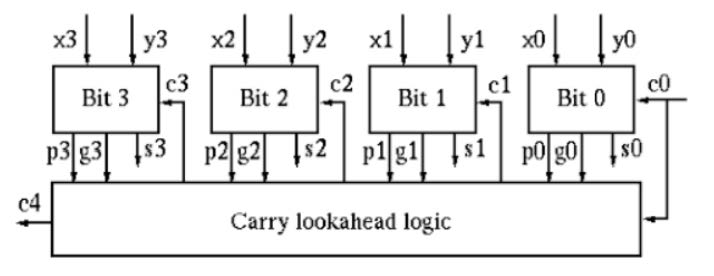
\includegraphics{assets/CarryLookAheadAdder.jpg}
    \end{figure} 
\end{problem}

\begin{problem}{Answer the following questions}
    \begin{enumerate}
        \item Describe the statement assign (continuous assignment).
        \item Define, give examples of expressions, operands, operator in DataFlow Modeling.
        \item List the types of operators used in DataFlow Modeling (arithmetic, logical, relational, equality, bitwise, reduction, shift, concatenation, and conditional), give examples.
        \item Instruction: 6.1 Continuous Assignments,6.3 Expressions , Operators, and Operands, 6.4 Operator Types–Chapter 6. Dataflow Modeling–Verilog HDL Samir
    \end{enumerate}
\end{problem}

\end{document}